\subsection{RMN: Corrimiento químico de $^7$Li}

\begin{figure}[h!]
    \centering
    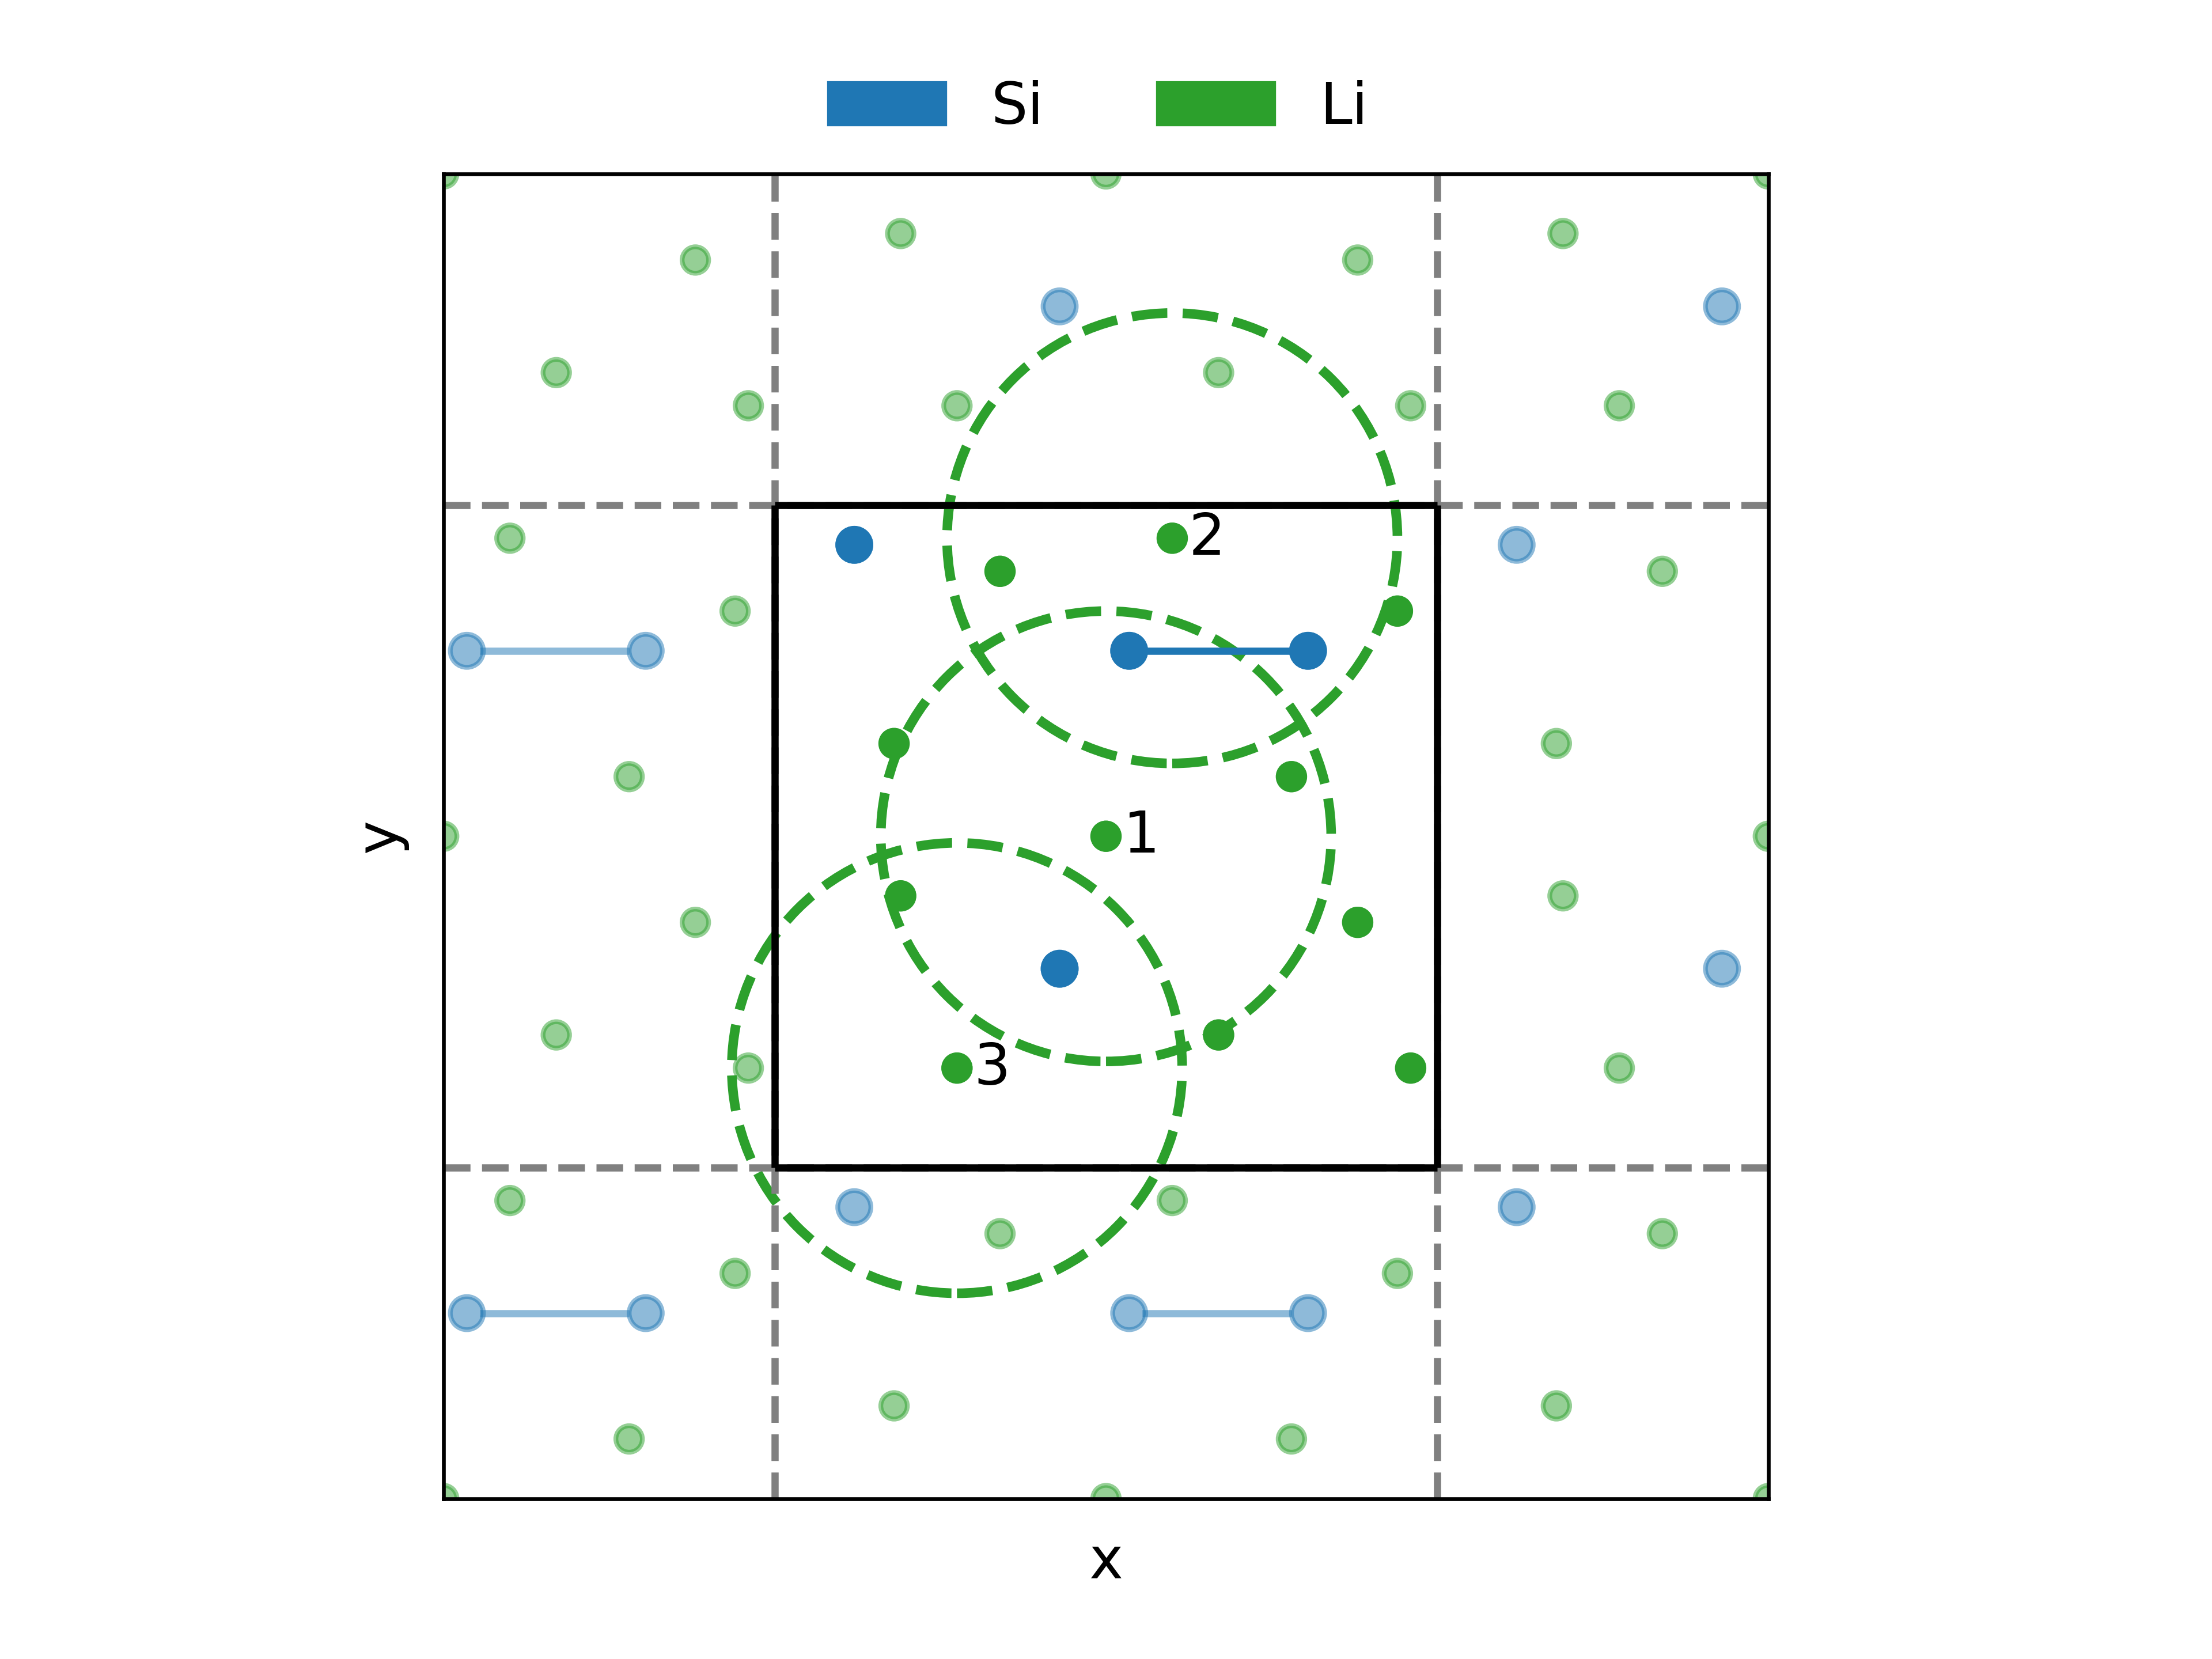
\includegraphics[width=.7\textwidth]{Silicio/prediccion/resultados/nmr/viz.png}
    \caption{Diagrama para explicar el modelo de primeros vecinos que predice los
    espectros de RMN en sistemas Li--Si.} 
    \label{fig:viz}
\end{figure}

\begin{figure}[h!]
    \centering
    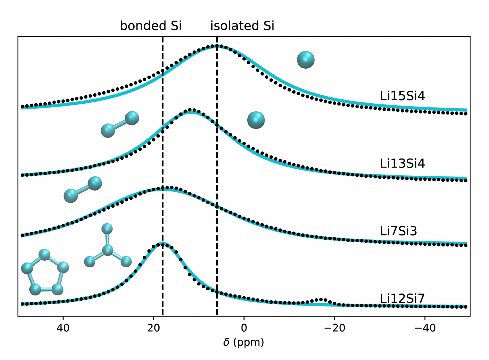
\includegraphics[width=.7\textwidth]{Silicio/prediccion/resultados/nmr/c-nmr.png}
    \caption{Espectros de corrimiento químico de $^7$Li para aleaciones 
    cristalinas. Los puntos corresponden a las mediciones de Key \textit{et al.}
    y las líneas al modelo de primeros vecinos. Las líneas verticales indican las 
    contribuciones del Si enlazado y aislado. Las barras de error son menores que
    el ancho de las líneas.}
    \label{fig:c-nmr}
\end{figure}

\begin{figure}[h!]
    \centering
    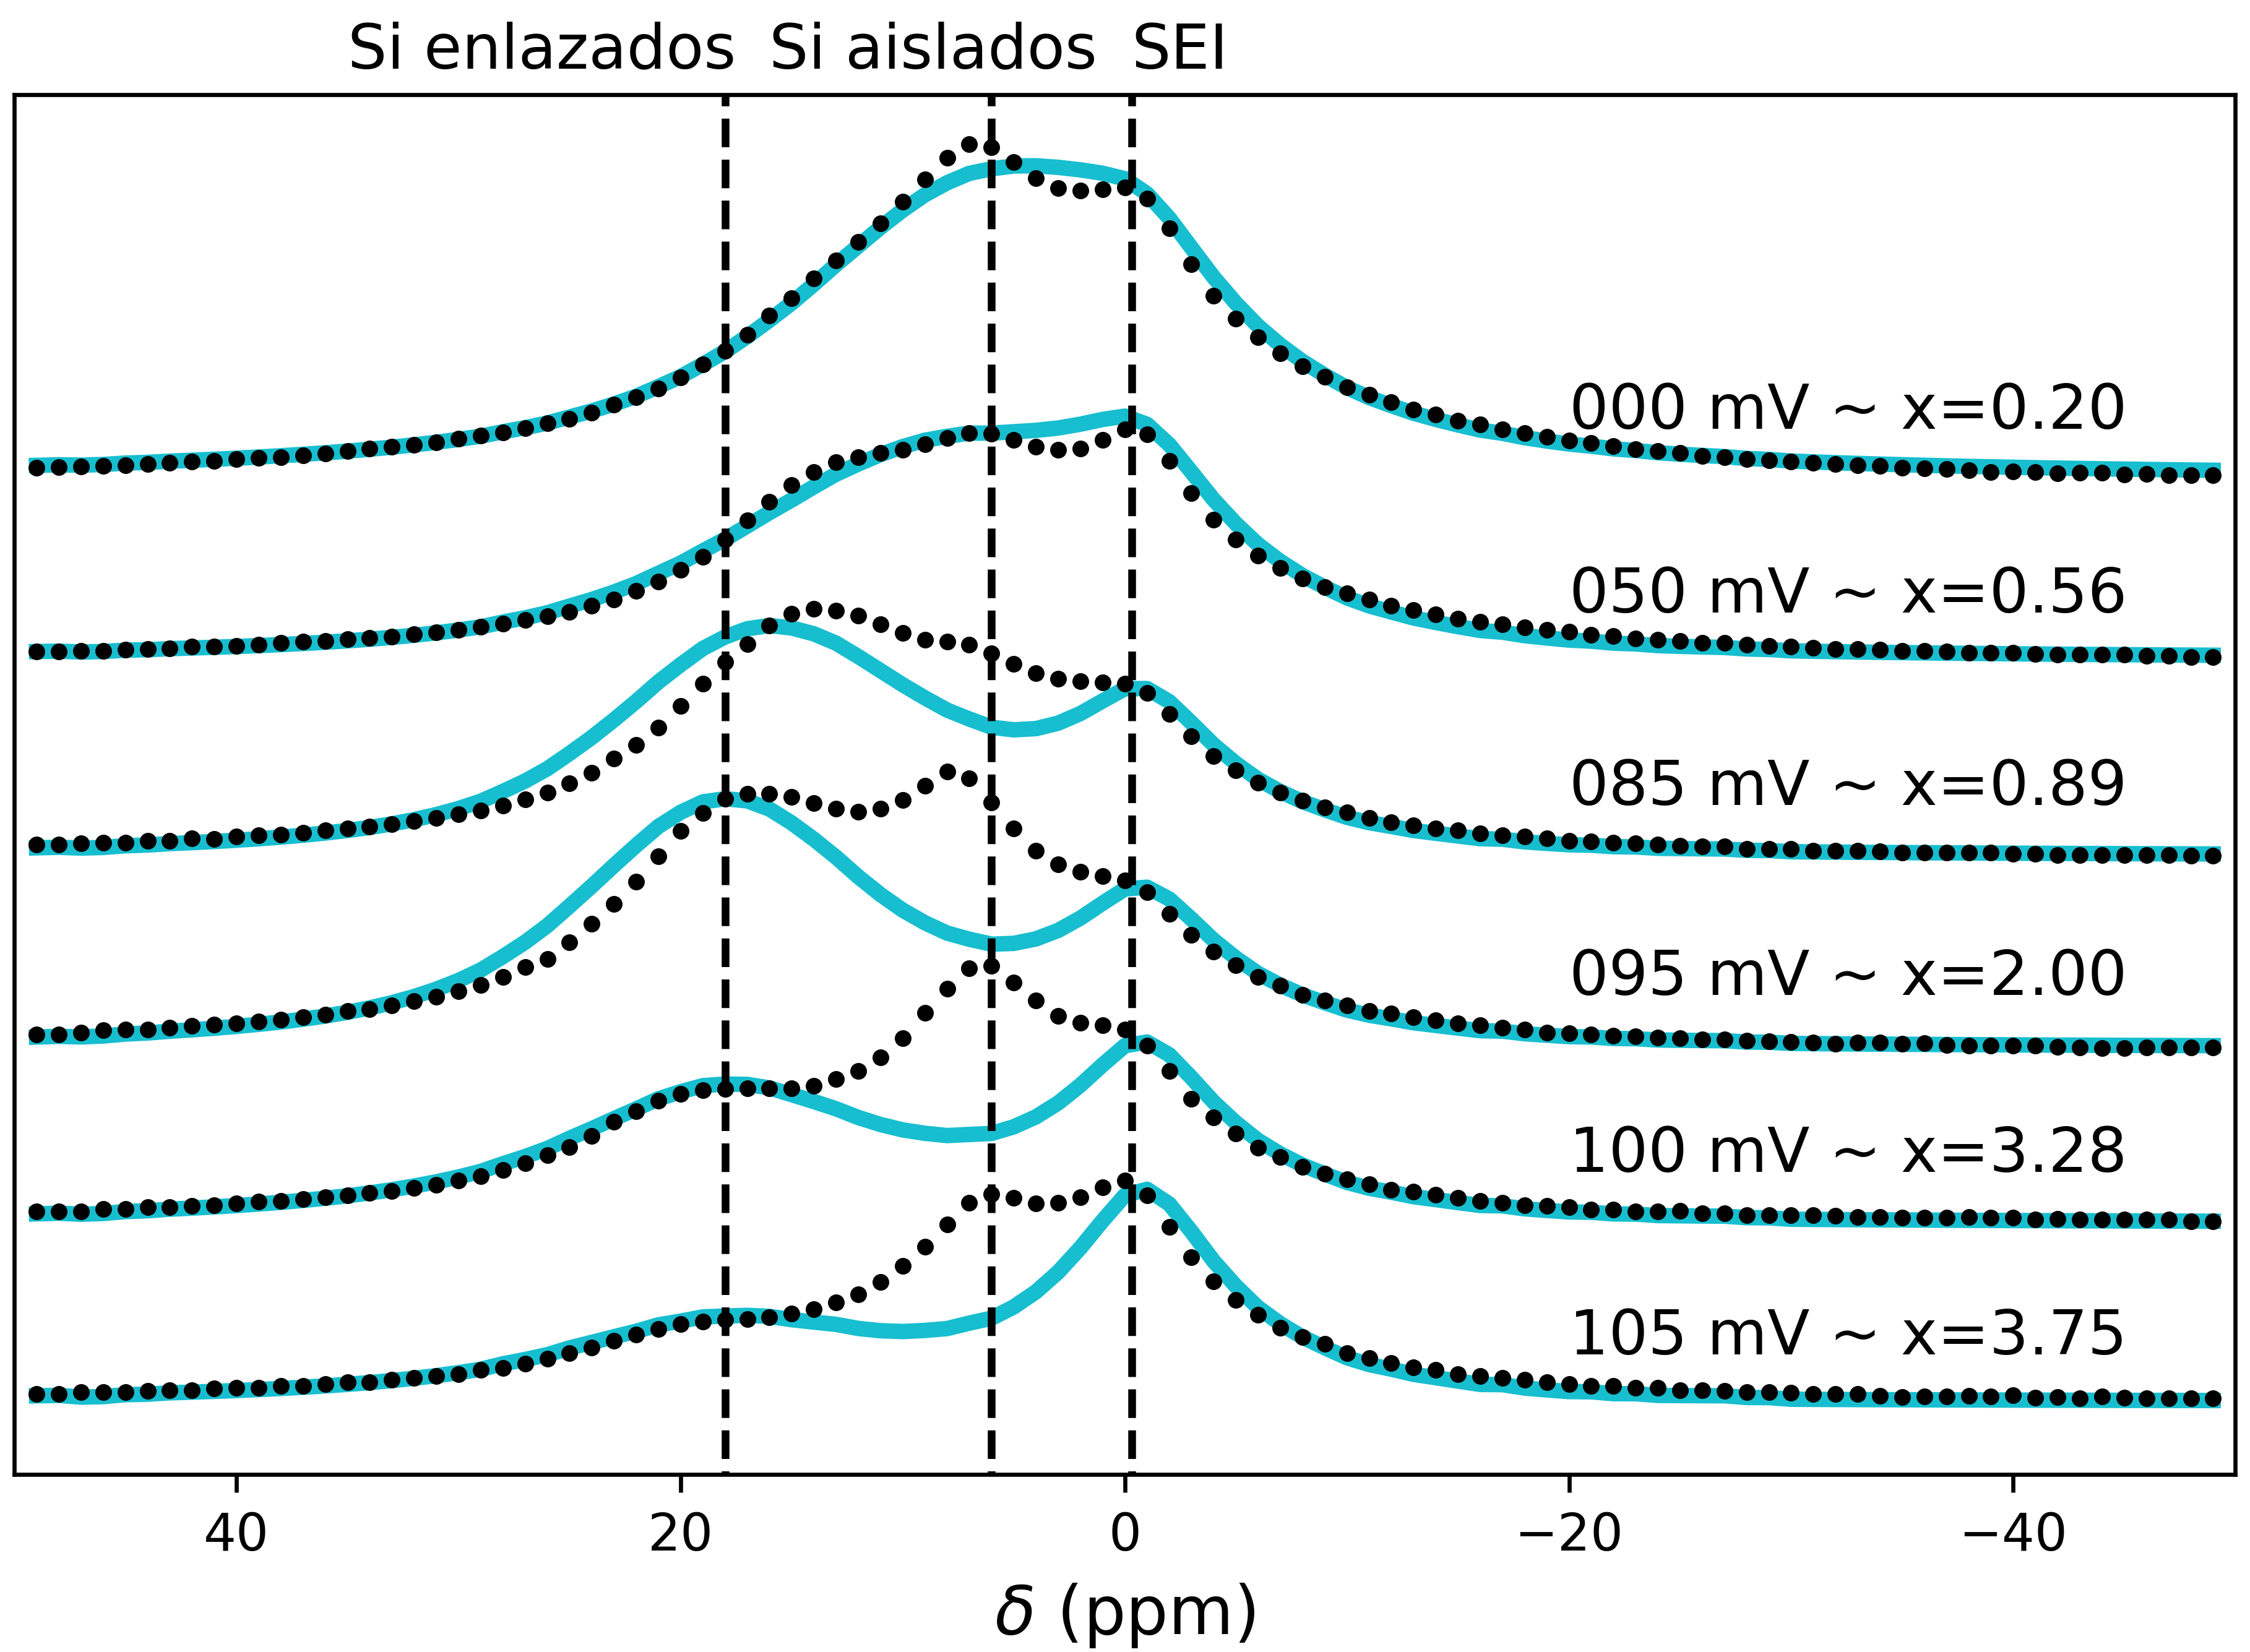
\includegraphics[width=.7\textwidth]{Silicio/prediccion/resultados/nmr/a-nmr.png}
    \caption{Espectros de corrimiento químico de $^7$Li para estructuras amorfas.
    Los puntos corresponden a las mediciones de Key \textit{et al.}. Los 
    resultados del modelo se representan con líneas continuas y se añade una 
    contribución de la SEI para comparar con el experimento. Las líneas verticales 
    indican las contribuciones de la SEI y de los átomos de Si enlazados o 
    aislados. Las barras de error son menores que el ancho de las líneas. Las 
    discrepancias a 6 ppm pueden deberse a una litiación inhomogénea en los 
    experimentos, como se explica en la referencia TODO.} 
    \label{fig:a-nmr}
\end{figure}
